%%%%% Beginning of preamble %%%%%

\documentclass[12pt]{article}  %What kind of document (article) and what size
\usepackage[document]{ragged2e}

\usepackage{wrapfig}
%Packages to load which give you useful commands
\usepackage{graphicx}
\usepackage{amssymb, amsmath, amsthm}
\usepackage{fancyhdr}
\usepackage[linguistics]{forest}
\usepackage{enumerate}
%\usepackage{enumerate}
\usepackage[margin=1in]{geometry} 
\pagestyle{fancy}
\fancyhf{}
\lhead{MA 583: HW1, \today, Discussion A4}
\rhead{Benjamin Draves}


\renewcommand{\headrulewidth}{.4pt}
\renewcommand{\footrulewidth}{0.4pt}

\topmargin = -0.4 in
%\headheight = 0.0 in t
%\headsep = .3 in
\parskip = 0.2in
%\parindent = 0.0in

%%%%%%%%%%new commands%%%%%%%%%%%%
\newcommand{\N}{{\mathbb{N}}}
\newcommand{\Z}{{\mathbb{Z}}}
\newcommand{\R}{{\mathbb{R}}}
\newcommand{\Q}{{\mathbb{Q}}}
\newcommand{\e}{{\epsilon}}
\newcommand{\del}{{\delta}}
\newcommand{\m}{{\mid}}
\newcommand{\infsum}{{\sum_{n=1}^\infty}}
\newcommand{\la}{{\langle}}
\newcommand{\ra}{{\rangle}}
\newcommand{\E}{{\mathbb{E}}}
\newcommand{\V}{{\mathbb{V}}}
\newcommand{\prob}{{\mathbb{P}}}
%defines a few theorem-type environments
\newtheorem{theorem}{Theorem}
\newtheorem{corollary}[theorem]{Corollary}
\newtheorem{definition}{Definition}
\newtheorem{lemma}[theorem]{Lemma}
%%%%% End of preamble %%%%%

\begin{document}

\begin{description}
\item[Exercise 1.2.4] 
\begin{enumerate}[(a)]
	\item The distribution function for $Z$ is given by $F_Z(z) = \prob(Z\leq z)$. This gives \[F_Z(z) = \begin{cases} 
    0 & x< 0 \\
    1/4 & 0\leq z < 1\\
	3/4 & 1\leq z < 2\\
	7/8 & 2\leq z < 3\\
	1 & 3\leq z\\
   \end{cases}
\] 
\begin{figure}[h!]
  \centering
    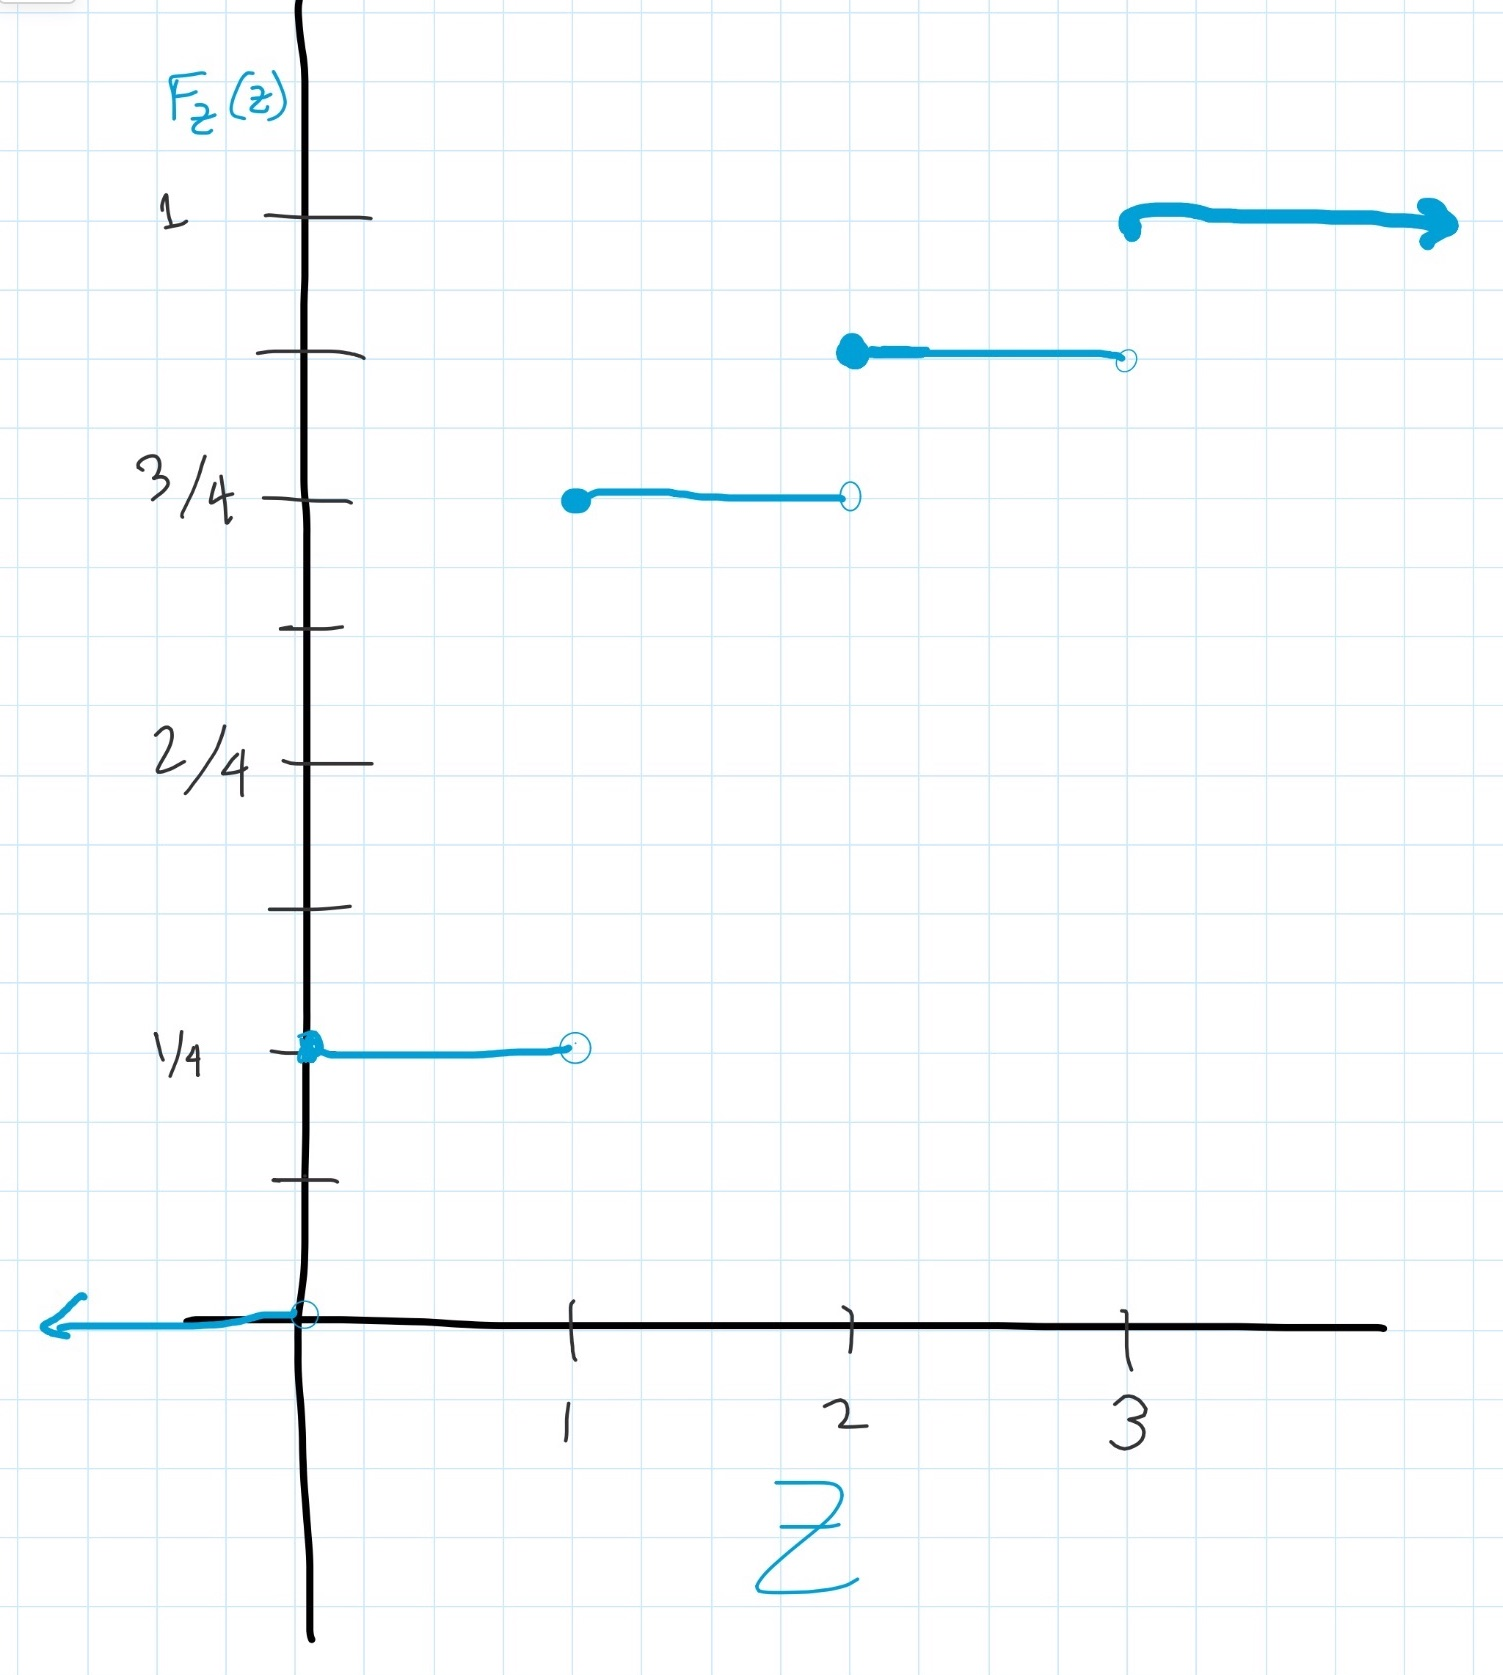
\includegraphics[width=0.48\textwidth]{CDF.jpg}
\end{figure}
\item \begin{align*}
\E(Z) &= 0\prob(Z = 0) + 1\prob(Z = 1) + 2\prob(Z = 2) + 3\prob(Z = 3)\\
	  &= 0 + 1/2 + 1/4 + 3/8\\
	  &= 9/8
\end{align*}
\item \begin{align*}
\E(Z^2) &= 0\prob(Z = 0) + 1\prob(Z = 1) + 4\prob(Z = 2) + 9\prob(Z = 3)\\
	  &= 0 + 1/2 + 1/2 + 9/8\\
	  &= 17/8
\end{align*}
\begin{align*}
\V(Z) &= \E(Z^2) - [\E(Z)]^2 = 17/8 - 81/64 = 55/64
\end{align*}
\end{enumerate}
\item[Exercise 1.2.9] (Distribution Function) Suppose that $x\leq 1$. Then we have 
$$F_X(x) = \int_{-\infty}^{x}f(y)dy =  \int_0^x ydy = \frac{1}{2}x^2$$ Now suppose that $x>1$. Then 
$$F_X(x) = \int_{-\infty}^{x}f(y)dy =  \int_0^1 xdy  + \int_{1}^x(2-y)dy = 1/2 + -\frac{1}{2}x^2+2x -3/2 = -\frac{1}{2}x^2 + 2x -1$$ Therefore, we have \[F_x(x) = \begin{cases} 
    0 & x< 0 \\
    \frac{1}{2}x^2 & 0\leq x \leq 1\\
	-\frac{1}{2}x^2 + 2x -1 & 1< x \leq 2\\
	1 & 2<x
   \end{cases}
\] 
(Mean) 
\begin{align*}
\E(X) &= \int_0^2xf(x)dx = \int_0^1x^2dx + \int_1^2 (2x - x^2)dx\\
&= \frac{1}{3}x^3\Big\vert_0^1 + x^2\Big\vert_1^2 - \frac{1}{3}x^3\Big\vert_1^2 = \frac{1}{3} + 3 - \frac{7}{3} = 1  
\end{align*}
(Variance)\begin{align*}
\E(X^2) &= \int_0^2x^2f(x)dx = \int_0^1x^3dx + \int_1^2 (2x^2 - x^3)dx\\
&= \frac{1}{4}x^4\Big\vert_0^1 + \frac{2}{3}x^3\Big\vert_1^2 - \frac{1}{4}x^4\Big\vert_1^2 = \frac{1}{4} + \frac{14}{3} - \frac{15}{4} = \frac{7}{6}\\
\V(X) & = \E(X^2) - [\E(X)]^2 = \frac{7}{6} - 1^2 = \frac{1}{6}  
\end{align*}
\item[Exercise 1.3.5] Let $N$ be the number of bacteria in a portion of a slide where $N\sim\text{Pois}(5)$. Then \begin{align*}P(N\geq 8) &= 1 - P(N\leq 7) = 1 - \sum_{n = 0}^{7}P(N = n) = 1 - \sum_{n = 0}^{7}\frac{5^ne^{-5}}{n!}\\
&= 1 - e^{-5}\Big(\frac{5^0}{0!} + \frac{5^1}{1!} +\ldots +\frac{5^7}{7!}\Big) \approx 0.133
\end{align*}
\item[Problem 1.4.2 (a)] Let $W\sim\text{Exp}(\theta)$ and denote $\mu = \frac{1}{\theta}$. Then 
\begin{align*}
\prob(W>\mu) = \int_{\mu}^{\infty} \theta e^{-\theta x}dx = -e^{-\theta x}\Big\vert_{\mu}^{\infty} = 0 + e^{-\theta\mu} = e^{-1}
\end{align*}
\item[Problem 1.5.2] Let $Z = \min(X_1, X_2, \ldots, X_n)$. Then we have 
\begin{align*}
F_Z(z) &= \prob(Z\leq z) = 1- \prob(Z>z) = 1 - \prob(X_1>z, \ldots, X_n>z) \overset{i.i.d}{=} 1 -[\prob(X_1>z)]^n\\
&= 1 - [1 - \prob(X_1\leq z)]^n = 1 - [e^{-\lambda z}]^n = 1 - e^{-n\lambda z}
\end{align*} This shows that $Z\sim\text{Exp}(n\lambda)$

\item[Exercise 2.1.5] Suppose that $X\sim\text{Pois}(\lambda)$. Let $A = \{X = 2n+1: n\in\N\}$ be the event that $X$ is odd. Then we have $$\E(X|A) = \sum_{n=0}^{\infty}n\prob(X = n|A) = \sum_{n= 0}^{\infty}n\frac{\prob(X = n, A)}{\prob(A)}$$ First we find $\prob(A)$. 
\begin{align*}
\prob(A) &= \sum_{k=0}^{\infty}\frac{\lambda^{2k+1}e^{-\lambda}}{(2k+1)!} = e^{-\lambda}\sum_{k=0}
^{\infty}\frac{\lambda^{2k+1}}{(2k+1)!} = e^{-\lambda}\sinh(\lambda)
\end{align*}
Now notice that $\prob(X = n, A) = 0$ if $n$ is even. If $n$ is odd, then $\prob(X = n, A) = \frac{e^{-\lambda}\lambda^n}{n!}$. This gives a reduction in our expression to 
\begin{align*}
\E(X|A) &= \sum_{n odd}n\frac{e^{-\lambda}\lambda^n/n!}{e^{-\lambda}\sinh(\lambda)} = \frac{1}{\sinh(\lambda)}\sum_{k=0}^{\infty}(2k+1)\frac{\lambda^{2k+1}}{(2k+1)!}\\ 
&= \frac{\lambda}{\sinh(\lambda)}\sum_{k=0}^{\infty}\frac{\lambda^{2k}}{(2k)!} = \lambda\frac{\cosh(\lambda)}{\sinh(\lambda)} = \lambda\coth(\lambda)
\end{align*}

\item[Problem 2.1.1] 
\begin{enumerate}[(a)]
\item Suppose that $M\sim\text{Binom}(N,p)$ and $X|M\sim\text{Binom}(N,\pi)$. Then we have 
\begin{align*}
\prob(X = x) &= \sum_{m}\prob(X=x, M=m) = \sum_{m}\prob(X=x|M=m)\prob(M=m)\\
&= \sum_{m=x}^{N}\binom{m}{x}\pi^{x}(1-\pi)^{m-x}\binom{N}{m}p^m(1-p)^{N-m}\\ 
&= \frac{N!\pi^{x}}{x!}\sum_{m=x}^{N}\frac{(1-\pi)^{m-x}p^m(1-p)^{N-m}}{(m-x)!(N-m)!}\\
&= \frac{N!\pi^{x}}{x!}\sum_{k=0}^{N-x}\frac{(1-\pi)^{k}p^{k+x}(1-p)^{N-m-k}}{k!(N-m-k)!}\\
&= \frac{N!\pi^{x}}{x!(N-x)!}\sum_{k=0}^{N-x}\frac{(N-x)!}{k!(N-m-k)!}(1-\pi)^{k}p^{k+x}(1-p)^{N-m-k}\\
&= \frac{N!(p\pi)^{x}}{x!(N-x)!}\sum_{k=0}^{N-x}\binom{N-x}{k}[(1-\pi)p]^{k}(1-p)^{N-m-k}\\
&= \binom{N}{x}(p\pi)^x[(1-\pi)p + (1-p)]^{N-x}\\
&= \binom{N}{x}(p\pi)^x(1-p\pi)^{N-x}\\
\end{align*}
Which we recognize as the Binomial pmf. Hence the marginal distribution of $X$ is given by $X\sim\text{Binom}(N,p\pi)$

\item 
\begin{align*}
Cov(X,M-X) &= Cov(X,M) - Cov(X,X) \\
&= \E(XM) - \E(X)\E(M) - \V(X)\\
&= \E[\E(XM|M)] - N^2p^2\pi - Np\pi(1-p\pi)\\
&= \E[M\E(X|M)]- N^2p^2\pi - Np\pi(1-p\pi)\\
&= \E[M^2\pi]- N^2p^2\pi - Np\pi(1-p\pi)\\
&= \pi[\V(M) + \E(M)^2]- N^2p^2\pi - Np\pi(1-p\pi)\\
&= \pi[Np(1-p) + N^2p^2]- N^2p^2\pi - Np\pi(1-p\pi)\\
&= Np(1-p)\pi + N^2p^2\pi- N^2p^2\pi - Np\pi(1-p\pi)\\
&= Np\pi(1-p  - 1+p\pi)\\
&= Np\pi(-p +p\pi)\\
&= Np^2\pi(\pi-1)\\
\end{align*}
\end{enumerate}


\item[Problem 2.1.7] Let $A$ be the event that an airplane crash was diagnosed as due to a structural failure and $B$ be the event that an airplane crash was due to a structural failure. Then we look to find $\prob(B|A)$. Using Bayes' Law we have 
\begin{align*}
\prob(B|A) = \frac{\prob(A|B)\prob(B)}{\prob(A)} = \frac{\prob(A|B)\prob(B)}{\prob(A|B)\prob(B) + \prob(A|B^C)\prob(B^C)}
 \end{align*} 
From the given, we know that $\prob(A|B) = 0.85$, $\prob(A|B^C) = 0.35$, $\prob(B) = 0.3$, $\prob(B^C) = 0.7$. Using this information gives our solution, 

\begin{align*}
\prob(B|A) = \frac{(0.85)(0.3)}{(0.85)(0.3) + (0.35)(0.7)} = 0.51
 \end{align*}


\end{description}	
\end{document} 


